\newpage
\section{Lösungskonzept}
\subsection[Designkonzept]{Designkonzept}
Das Design des Admin-UIs wurde von einem seperaten Designerteam erstellt, welches nah mit dem Kunden zusammengearbeitet hat.

Das Designteam hat dann Mockups für die verschiedenen Seiten und Seitenelemente erstellt: \\\\
\textit{Notiz: Um die Anonymität des Kunden zu wahren, wurden einige Stellen der Mockups geschwärzt.}

Die Mockups orientieren sich an den Anforderungen \hyperref[Tab:A4]{A4}, \hyperref[Tab:A5]{A5}, \hyperref[Tab:A6]{A6} und \hyperref[Tab:A7]{A7}. Sie fügen jedoch noch andere Elemente hinzu, um für ein gutes UX zu sorgen. Dazu gehörten: \\
\begin{itemize}
    \item Die Unterteilung der Eingabefelder mit der dazu passenden Überschrift.
    \item Platzhalter in den Eingabefeldern, um besser zu erkennen, was in die Felder eingetragen werden muss.
\end{itemize}
\subsubsection[Mockup für Seite zur Änderung des Projektowners]{Mockup für Seite zur Änderung des Projektowners}
\begin{figure}[H]
    \centering
    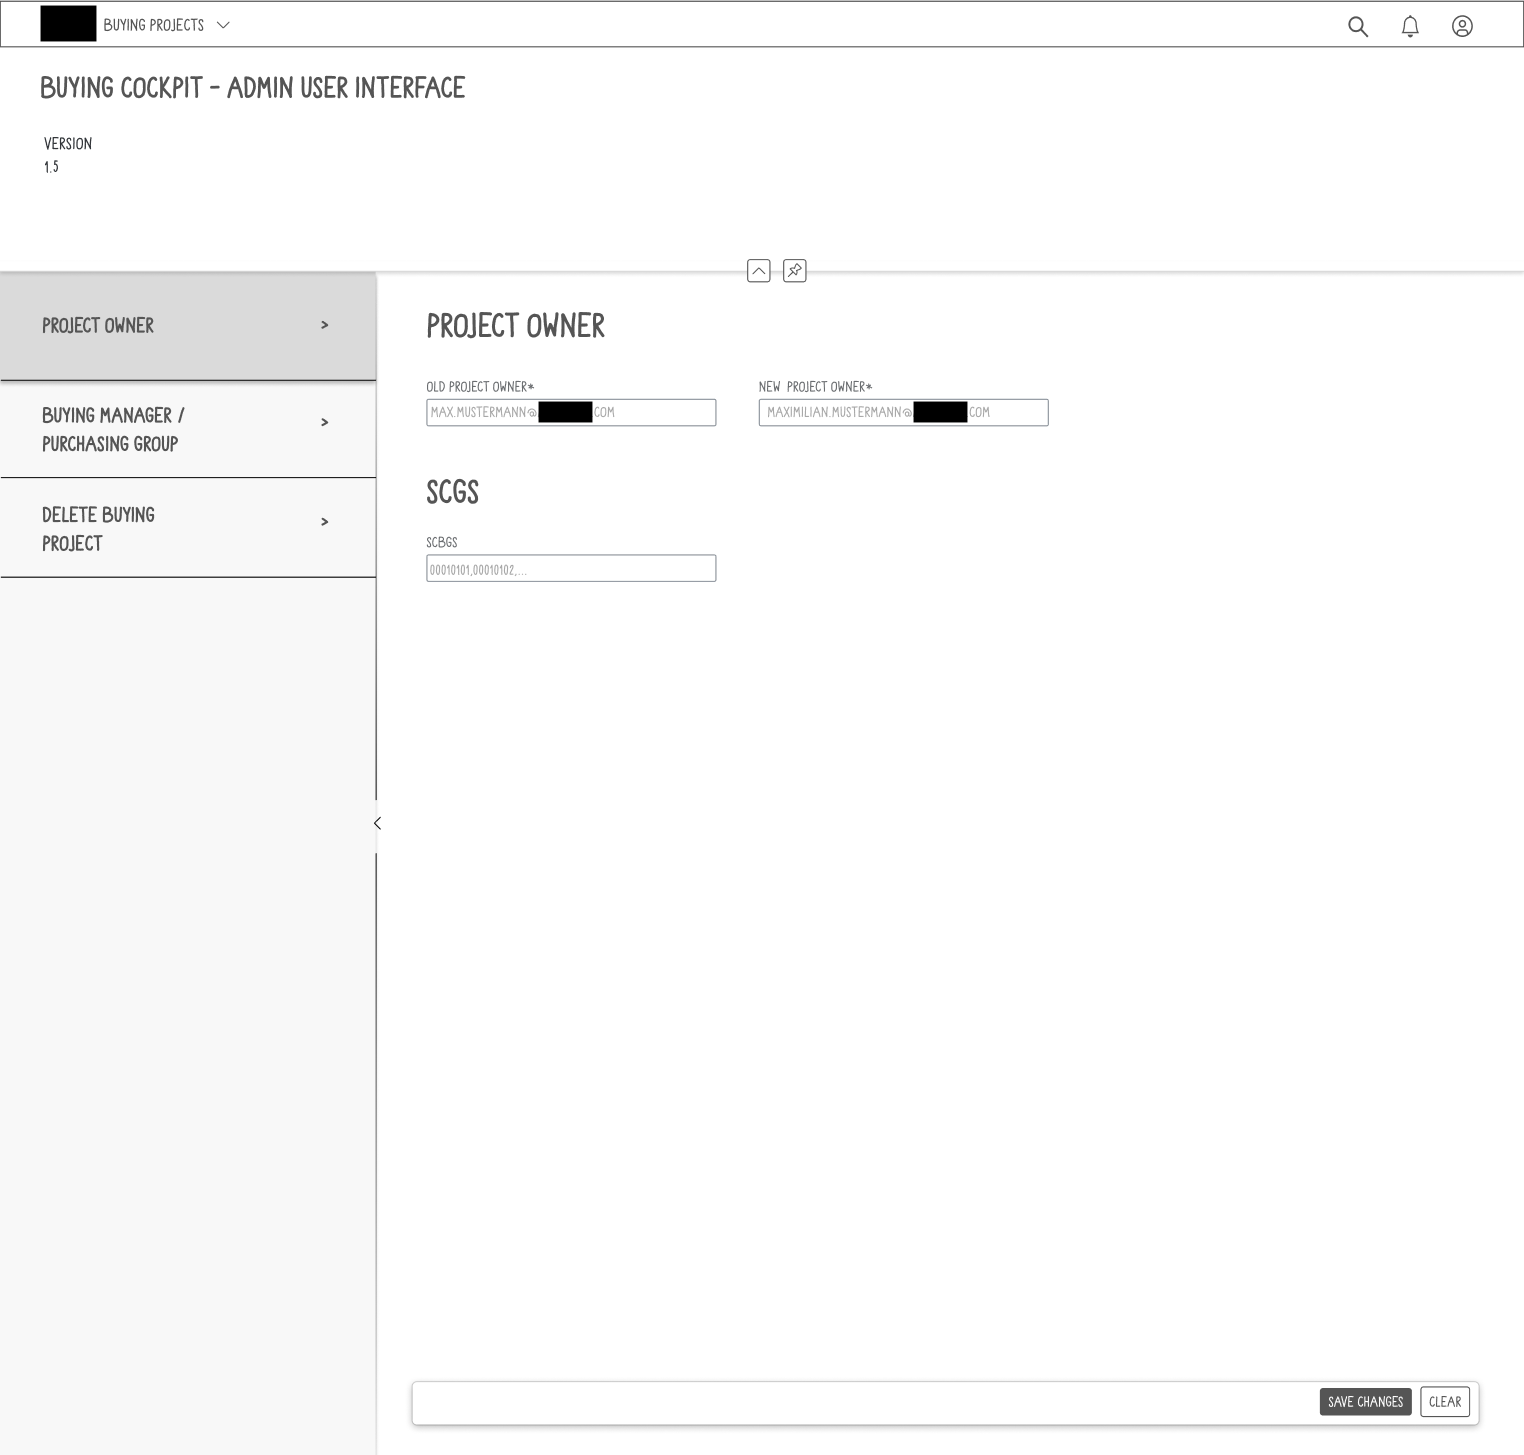
\includegraphics[width=\linewidth]{Images/Mockup_PO_anonym.png}
    \caption[Mockup: Admin-UI Projekowner Seite]{Mockup: Admin-UI Projekowner Seite}
\end{figure}

\subsubsection[Mockup für Seite zur Änderung des Projektmanagers und der Käufergruppe]{Mockup für Seite zur Änderung des Projektmanagers und der Käufergruppe}
\begin{figure}[H]
    \centering
    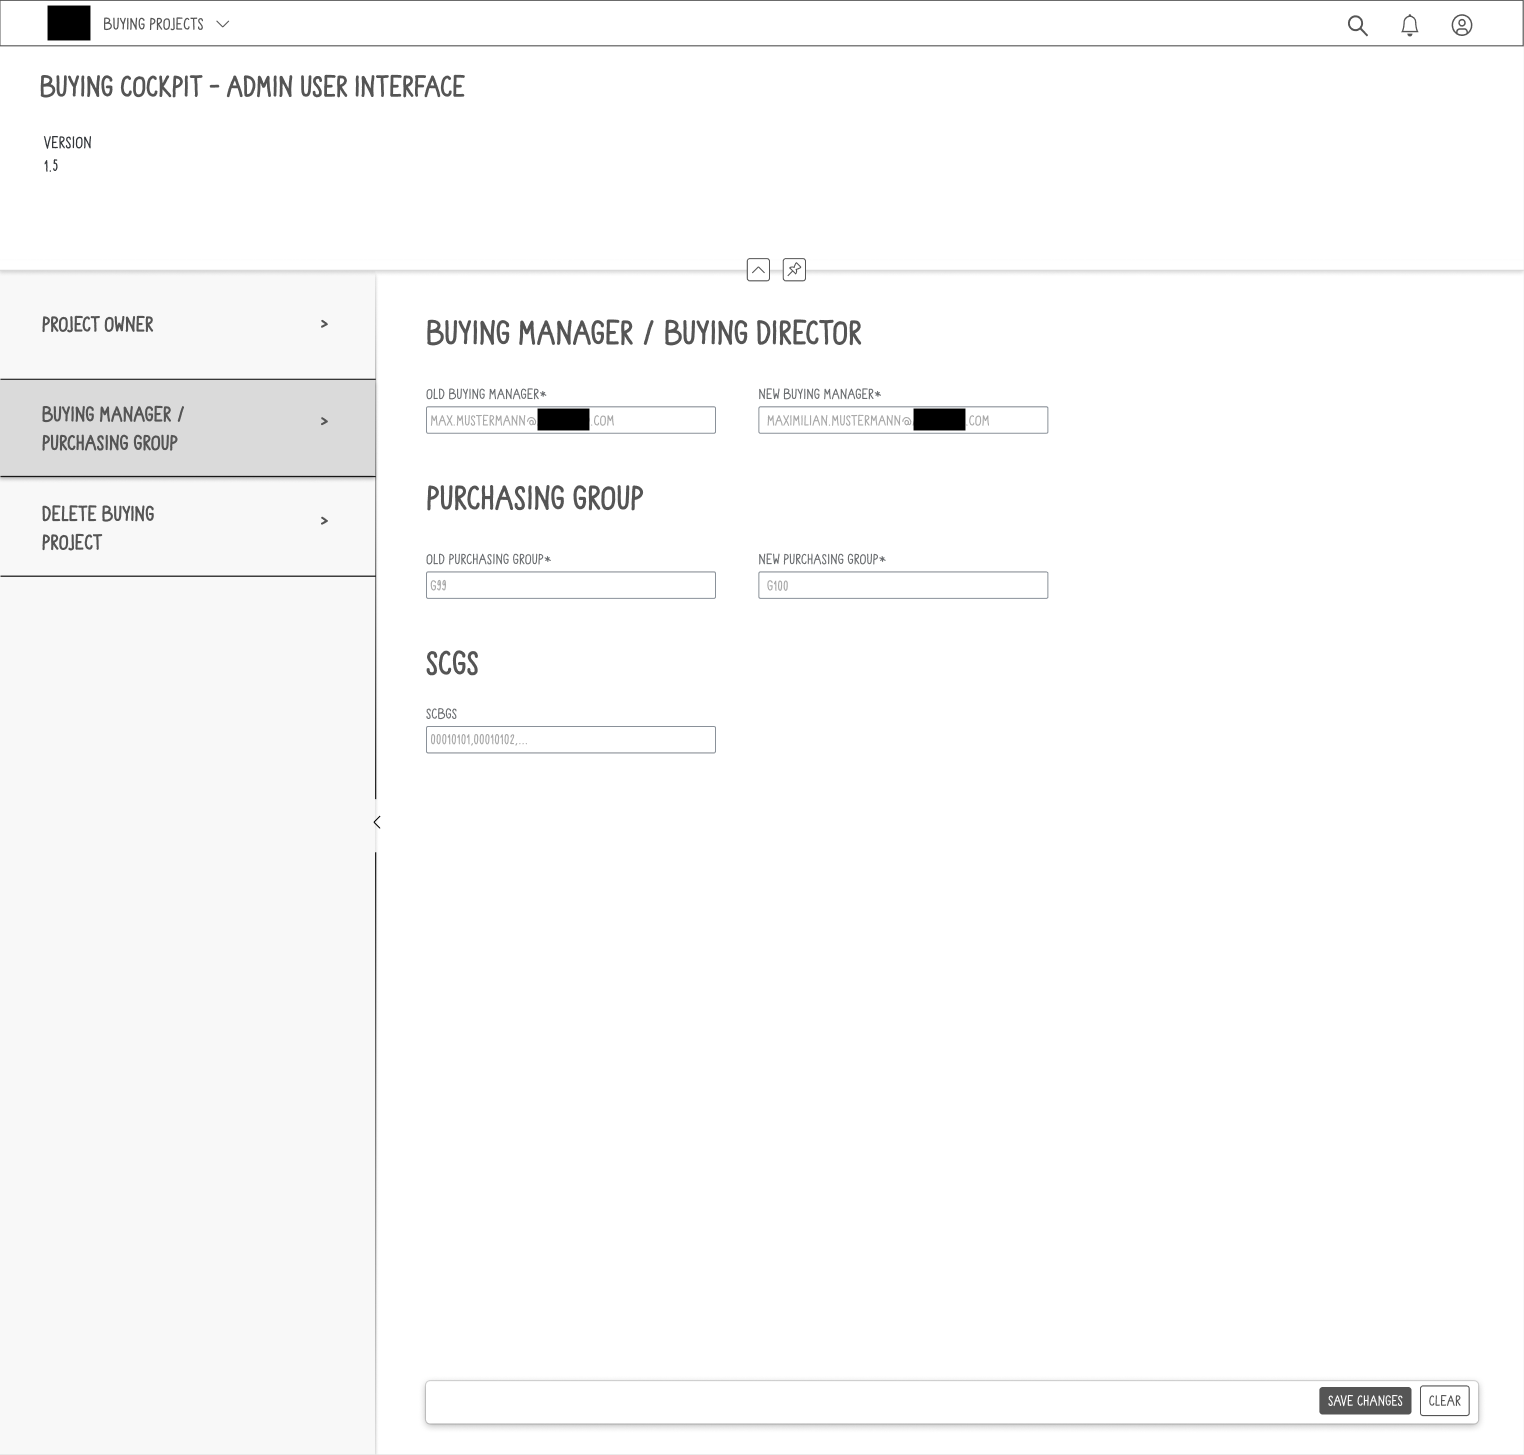
\includegraphics[width=\linewidth]{Images/Mockup_PM_anonym.png}
    \caption[Mockup: Admin-UI Projektmanager und Käufergruppe Seite]{Mockup: Admin-UI Projektmanager und Käufergruppe Seite}
\end{figure}

\subsubsection[Mockup für Seite zur Löschung von Projekten]{Mockup für Seite zur Löschung von Projekten}
\begin{figure}[H]
    \centering
    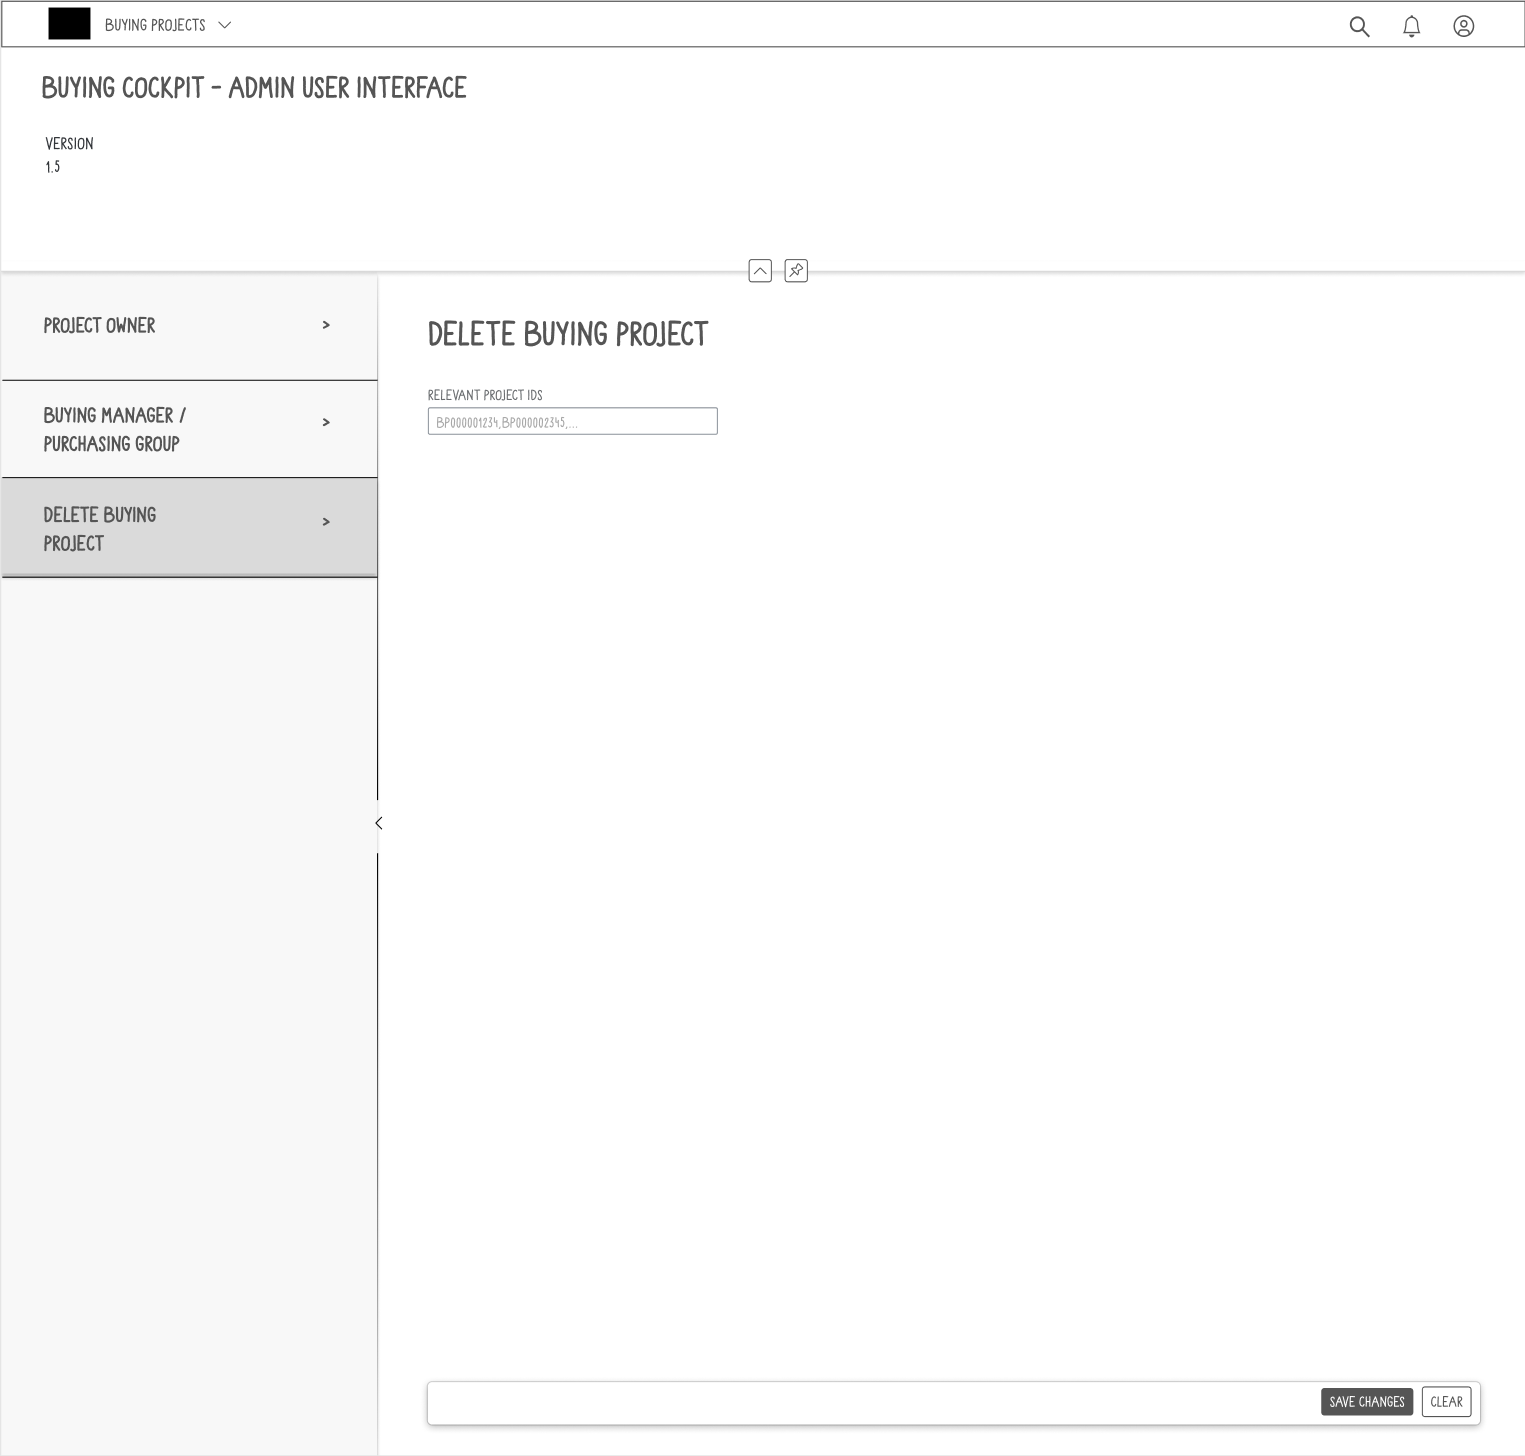
\includegraphics[width=\linewidth]{Images/Mockup_DEL_anonym.png}
    \caption[Mockup: Admin-UI Löschungs-Seite]{Mockup: Admin-UI Löschungs-Seite}
\end{figure}

\subsubsection[Mockup für Bestätigungs Pop-Up]{Mockup für Bestätigungs Pop-Up}
\begin{figure}[H]
    \centering
    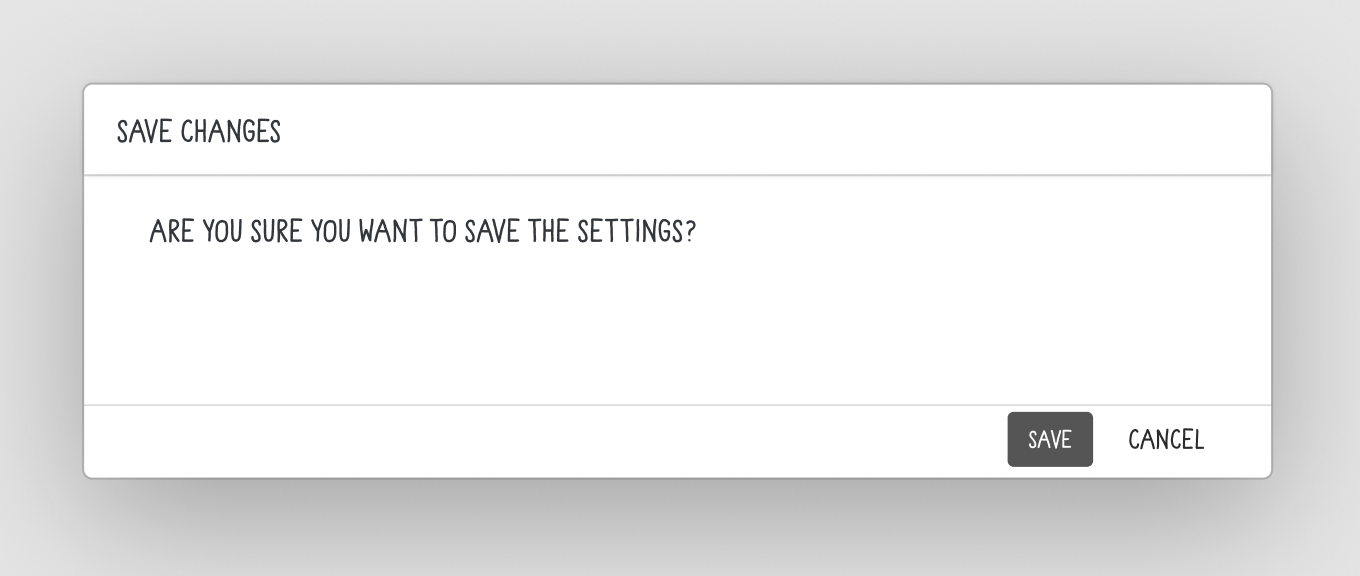
\includegraphics[width=\linewidth]{Images/Mockup_PopUp.png}
    \caption[Mockup: Admin-UI Pop-Up]{Mockup: Admin-UI Pop-Up}
\end{figure}





\subsection[Software-Design]{Software-Design}

